\documentclass{article}

% Packages
\usepackage[utf8]{inputenc} % UTF-8 input encoding
\usepackage[T1]{fontenc} % Font encoding
\usepackage{amsmath, amssymb} % Math packages
\usepackage{enumitem} % For customizing lists
\usepackage{lipsum} % For generating dummy text
\usepackage{listings}
\usepackage{graphicx}


\lstset{%
  language=bash,
  basicstyle=\fontfamily{pcr}\selectfont,
  commentstyle=\bfseries,
  escapeinside={(*@}{@*)}
}

\newcommand{\comment}[1]{\# here is a comment: #1}
\newcommand\floor[1]{\lfloor#1\rfloor}
\newcommand\ceil[1]{\lceil#1\rceil}

% Title and author information
\title{Algorithms (6470) HW05}
\author{Alex Darwiche}
\date{\today}

\begin{document}

\maketitle

\section*{Answers}

% Question 1
\subsection*{Q1}
\begin{enumerate}[label=(\alph*)]
    \item Yes, the $u.\pi$ can change for some $u \in V$. Assuming node $u$ is at depth $i$. 2 nodes at depth $i-1$ could both have an edge that connects to node $u$. The $u.\pi$ thus depends on which of those nodes you encounter first in your BFS. Thus, the order of the adjaceny matrix CAN affect $u.\pi$
    \item No, $u.d$ cannot change. A BFS looks through all the nodes away from the source, at each depth away from the source. This means that a BFS, even with ordering changed, will never change the $u.d$ of a node, because it would have found the shortest path in the first place, regardless of order.
\end{enumerate}

% Question 2
\subsection*{Q2}
\begin{enumerate}[label=(\alph*)]
    \item DFS on Figure 20.6:
    \subitem 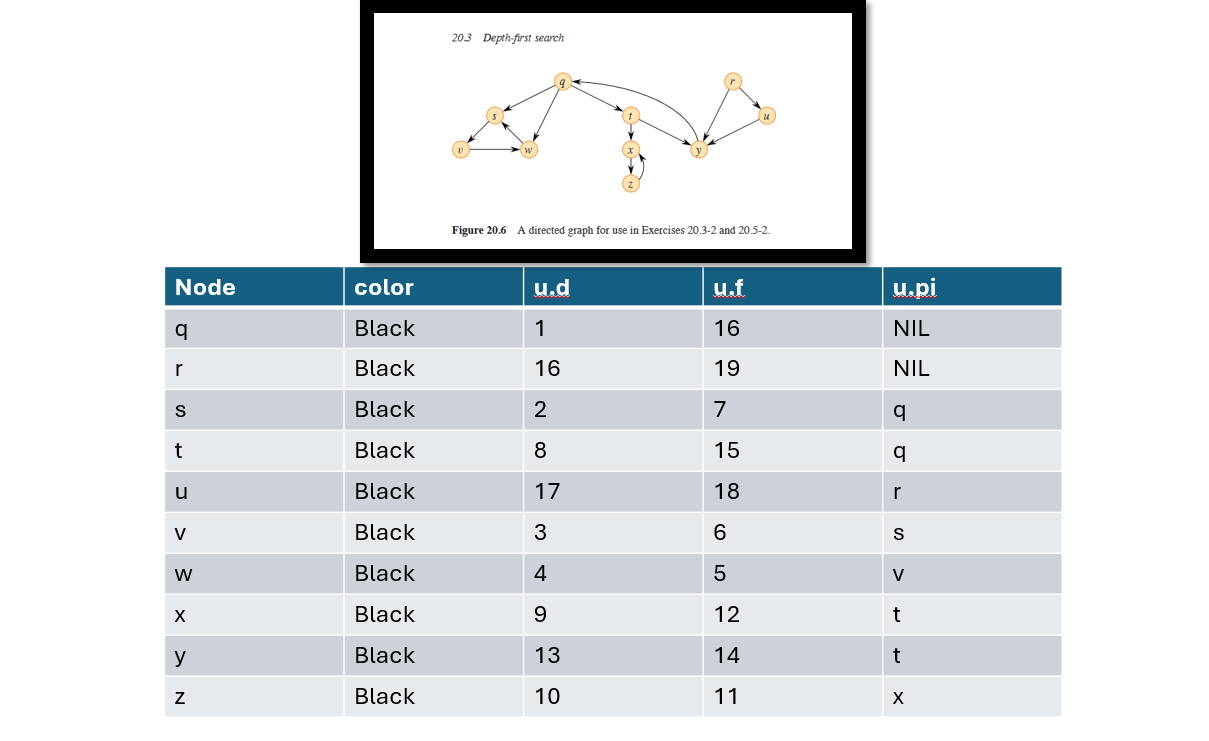
\includegraphics[width=1\textwidth]{dfs20.6.png}
    \subitem 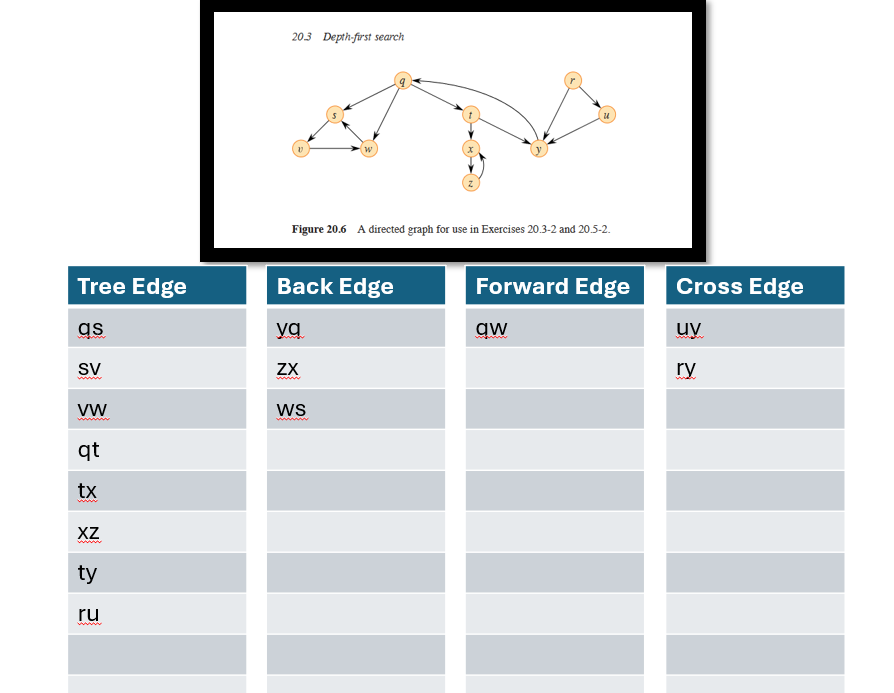
\includegraphics[width=1\textwidth]{classifications.png}
\end{enumerate}

% Question 3
\subsection*{Q3}
\begin{enumerate}[label=(\alph*)]
    \item This will always be true. If there is a path between nodes u and v, and u.d < v.d, then depth first search will search through all of u's child nodes until it explores the child that eventually connects to v. This means that v will always be a descendant of u, given the above assumptions.
\end{enumerate}

% Question 4
\subsection*{Q4}
\begin{enumerate}[label=(\alph*)]
    \item Topological Sort - alphabetical order
    \subitem 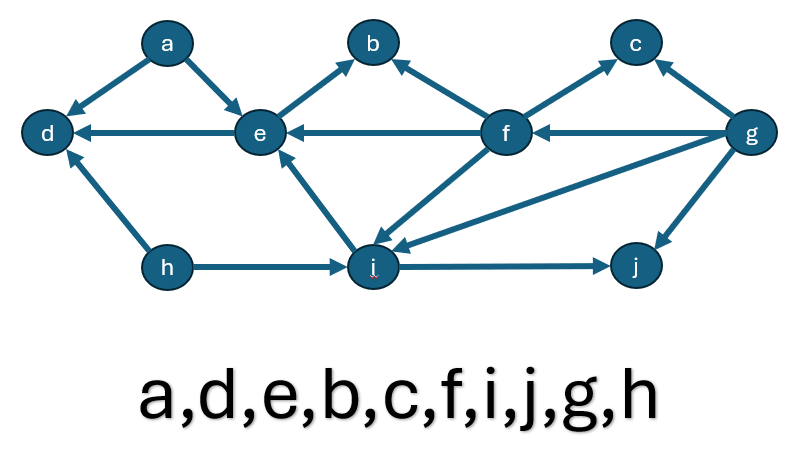
\includegraphics[width=.75\textwidth]{dfs.png}
\end{enumerate}

% Question 5
\subsection*{Q5}
\begin{enumerate}[label=(\alph*)]
    \item The first G1 shows how this algorithm can find the strongly connected components in a graph and distinguish them from other components. However, the second example illustrates how this cannot always work. The node B and C cannot reach one another if you begin at node C. This is not shown in the tables however, and illustrates why this algorithm does not work for all graphs.
    \subitem \includegraphics[width=.75\textwidth]{sssc.png}
\end{enumerate}

% Question 6
\subsection*{Q6}
\begin{enumerate}[label=(\alph*)]
    \item Kruskal Algorithm
    \subitem 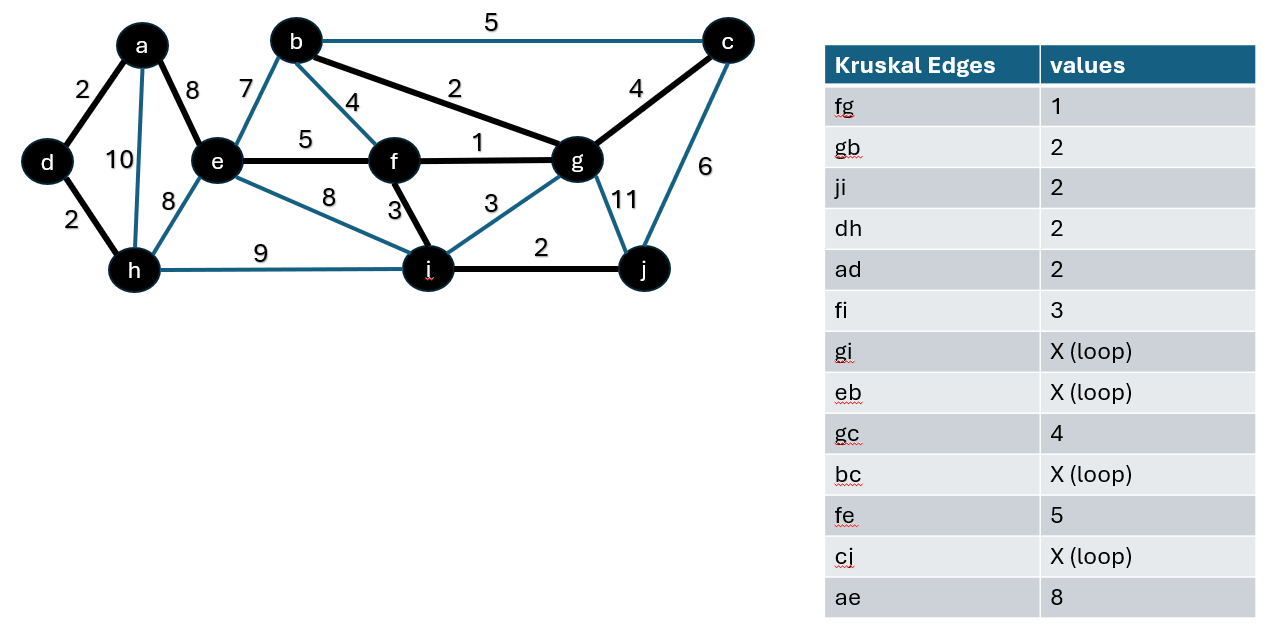
\includegraphics[width=.75\textwidth]{kruskal.png}
    \item Prim Algorithm
    \subitem 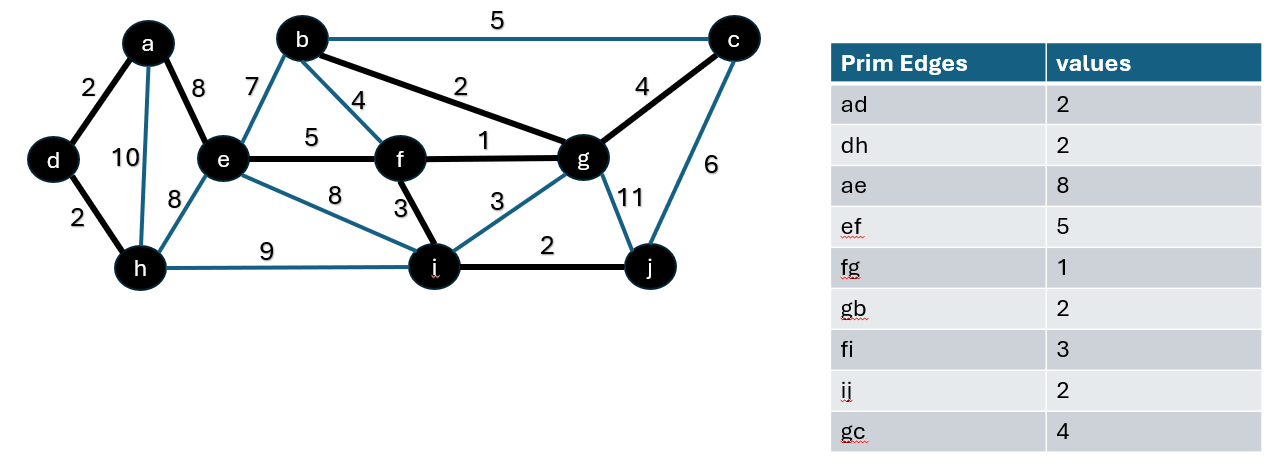
\includegraphics[width=.75\textwidth]{prims.png}
\end{enumerate}

% Question 7
\subsection*{Q7}
\begin{enumerate}[label=(\alph*)]
    \item To prove that an minimum weighted edge between u and v is part of some minimum spanning tree of G, I will use contradiction.
    \subitem (1) Assumption: There is a minimum spanning tree that does not include the edge from u to v, called S1.
    \subitem (2) Next, we will add in the edge from u to v to this tree.
    \subitem (3) This will now form a cycle in the graph.
    \subitem (4) To remove a loop, we first can look at all the different edges that make up the loop. A loop implies that every vertex in the loop has at least 2 edges coming from it. To remove this loop, we simply need to remove one of the edges that makes up said loop. To do this and maintain minimum spanning, we should remove the edge with the highest weight.
    \subitem (5) Now we remove an edge other than the one from u to v.
    \subitem (6) This leaves us with 2 different spanning trees. S1 and S2, where S2 is the minimum spanning tree that now includes the edge from u to v.
    \subitem (7) weight(S1) - weight(S2) > 0 or  weight(S1) > weight(S2) (THIS IS A CONTRADICTION)
    \subitem (8) This shows a contradiction as you can find a tree with a lower weight by including the edge from u to v. So by contradiction, the edge from u to v must be in some minimum spanning tree of graph G.
\end{enumerate}

% Question 8 (Graduate students only)
\subsection*{Q1 (Graduate students only)}
\begin{enumerate}[label=(\alph*)]
    \item Graph G
    \subitem 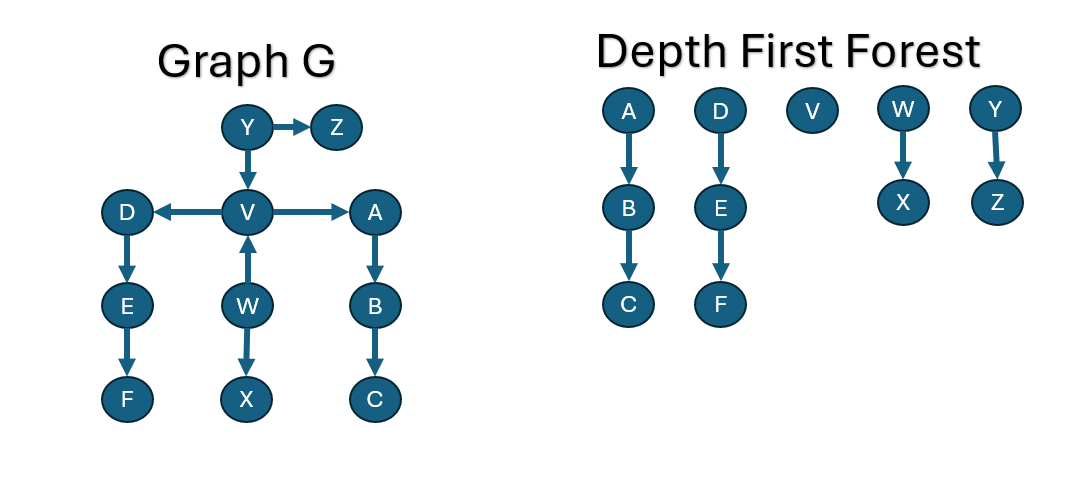
\includegraphics[width=.75\textwidth]{Grad1.png}
\end{enumerate}

% Question 9 (Graduate students only)
\subsection*{Q2 (Graduate students only)}
\begin{enumerate}[label=(\alph*)]
    \item This proof will be quite similar to the one used earlier in question 7.
    \subitem (1) First, assume that there exists a minimum spanning tree for graph G.
    \subitem (2) Now, we want to remove and edge and add an edge to this minimum spanning tree.
    \subitem (3) Case 1: Adding this edge increased the weight of the tree. This means that the new tree is not "minimum" spanning tree.
    \subitem (4) Case 2: Adding this edge decreased the weight of the tree. This means that the old tree is not "minimum" spanning tree.
    \subitem (5) In either case, we are able to conclude that once we've absolutely minimized the weight on the minimum spanning tree, any changes to the tree will only increase the weight of it, thus making it not minimum spanning. This means that there is only 1

    \item For a contradiction proof. 
    \subitem (1) Assume MST2 exist with an edge that is not in MST1, such that w(MST2) = w(MST1).
    \subitem (2) We will add an edge and remove an edge to form another spanning tree.
    \subitem (3) Case 1: We add an edge that increases the weight of MST2, such that w(MST2) > w(MST1)
    \subitem (4) Case 2: We add an edge that decreases the weight of MST2, such that w(MST2) < w(MST1)
    \subitem (5) Both cases are a contradiction, thus there is only 1 minimum spanning tree when all edges are unique.
\end{enumerate}


\end{document}
